\documentclass[spanish,12pt]{article}
\usepackage[spanish]{babel}
\usepackage[utf8]{inputenc}
\usepackage{xspace}
\usepackage{lmodern}
\usepackage{indentfirst}
\usepackage{xargs}
\usepackage{ifthen}
\usepackage{fancyhdr}
\usepackage{latexsym}
\usepackage{lastpage}
\usepackage{textcomp}
\usepackage{varwidth}
\usepackage{caratula, aed2-tad,aed2-symb,aed2-itef}
\usepackage{algorithmicx, algpseudocode, algorithm}
\usepackage{enumerate}
\usepackage{graphicx}
\usepackage{caption}
\usepackage{subcaption}
\usepackage{float}
\usepackage{anysize}
\marginsize{1.5cm}{1.5cm}{1.5cm}{1.5cm}

\begin{document}

\titulo{Informe 2}
\materia{Algoritmos y Estructuras de Datos III}
\author{Grupo  \\Alvarez Vico Jazm\'in\\Cortés Conde Titó Javier María\\Pedraza Marcelo \\ Rozenberg Uriel Jonathan}

\integrante {Jazmín Alvazer Vico}{75/15}{jazminalvarezvico@gmail.com}
\integrante {Marcelo Pedraza}{393/14}{marcelopedraza314@gmail.com}
\integrante {Uriel Jonathan Rozenberg}{838/12}{rozenberguriel@gmail.com}
\integrante {Javier María Cortés Conde Titó}{252/15}{javiercortescondetito@gmail.com}

\maketitle


\clearpage

\tableofcontents
\cleardoublepage

\section{Problema 1: Laberinto}

\subsection{Introducción}

En este problema los viajeros encuentran un mapa de un laberinto señalando algún lugar con una x sin embargo no todos los puntos están conectados. Ellos quisieran llegar a ese lugar caminando lo menos posible, además pueden esforzarse para romper una cantidad determinada de paredes. Nos piden que les informemos cuánto deben caminar de ser posible.

Formalmente esto equivale a modelar el problema utilzando un grafo que contiene nodos $"especiales"$(las paredes). Se busca la distancia entre dos nodos, pasando como mucho por p nodos especiales.

\subsection{Explicación de la solución}
Podemos dividir la resolución en tres partes: la primera, donde interpretamos la entrada y generamos un primer grafo, en el cual las habitaciones y paredes son nodos, y dos nodos son adyacentes si y sólo si sus casillas originales lo son. En la segunda parte vamos a copiar el primer grafo tantas veces como paredes se puedan romper, de manera que la acción de romper una pared esta representada por un cambio de nivel en el grafo. Así, cada nivel muestra cuantas paredes fueron atravesadas, y los $p-1$ nodos finales, los finales con p paredes atravesadas.

%Se podrá hacer un dibujo aca? la idea es hacer como un "plano" en perspectiva del primer grafo, como si fuese una feta de queso; y varias fetas abajo. ya fue igual

En la tercera parte, vamos a aplicar un bfs modificado, para calcular las distancias del nodo origen a todos los demás nodos. Entre las modificaciones se incluyen unos $"movimientos ilegales"$: estos son movimientos que el modelo solamente con  por un lado, no está permitido pasar a un nivel menor al que uno se encuentra. Además, no es correcto mover de un nodo $"habitación"$ a un nodo $"pared"$ en el mismo nivel.

Por último, se calcula la distancia mínima entre todos los nodos finales copiados. Si no existe un camino posible, el algoritmo devuelve -1



\subsection{Pseudocódico}

\subsubsection{Pseudocódigo}

\begin{algorithm}[H]{\textbf{solucion}(vector<Nodo>nodos, vector<Eje> ejes, int p)}
	\begin{algorithmic}[1]
		\State \quad res$\gets|nodos|$
		\State \quad vector$<Nodos>$ aux$\gets$nodos
		\State \quad Desde i=0 hasta i=p
			\State\quad \quad  respar$\gets$Bfs(aux)
			\State \quad \quad aux$\gets$ ClonarUltimoNivel(aux,ejes)
			\State \quad \quad Si respar$>$0 y respar$<$res hacer
				\State\quad \quad \quad  res$\gets$respar
			\State\quad \quad  finSi
		\State \quad finDesde
		\State \quad Si res=|nodos| hacer
			\State \quad \quad devovler -1
		\State \quad Sino
			\State \quad \quad  devolver res
		\State \quad finSi
	\end{algorithmic}
\end{algorithm}


\begin{algorithm}[H]{\textbf{Bfs}(vector<Nodos> nodos)}
	\begin{algorithmic}[1]
		\State \quad Para todo nodo i
			\State \quad \quad  pred(i)$\gets$-1, order(i)$\gets$-1
		\State \quad finPara
		\State \quad int next$\gets$ 0
		\State \quad lista list$\gets${(o,0)}
		\State \quad Mientras list$\neq \emtyset$ hacer
			\State \quad \quad Sacar un elemento (i,padre)
			\State \quad \quad pred(i,padre)=padre
			\State \quad \quad Si order(i=-1) hacer
				\State \quad \quad \quad order(i)$\gets$next
				\State \quad \quad \quad next+1
				\State \quad \quad \quad Para cada arista j conectada al nodo i hacer:
					\State \quad \quad \quad \quad Si(order(j)$=-1$ y nivel(j)$geq$nivel(i)) hacer
						 \State \quad \quad \quad \quad \quad list$\cup${(j,i)}
					\State \quad \quad \quad \quad finSi
				\State \quad \quad \quad   finPara
			\State \quad \quad  finSi
		\State \quad finMientras
		\State \quad int x $\gets$|nodos|-1, int res$\gets$2, int aux$\gets$0
		\State \quad Mientras $< |nodos|$ hacer
			\State \quad \quad  x$\gets$pred(x)
			\State \quad \quad Si x$\gets0 \ o \ x\gets-1$ cortar finSi
			\State \quad \quad res$\gets$res+1
			\State \quad \quad aux$\gets$aux+1
		\State \quad finMientras
		\State \quad Si x=-1
			\State \quad \quad devolver -1
		\State \quad Sino
			\State \quad \quad  devolver res
		\State \quad finSi




	\end{algorithmic}
\end{algorithm}

\begin{algorithm}[H]{\textbf{ClonarUltimoNivel}(aux,ejes)}
	\begin{algorithmic}[1]
		\State n <- ultimo nodo  de aux
		\State nivel <- n->nivel
		\State tamanioDelUltimoNivel
		\State mientras exista n  y n->nivel = nivel 
			\State retrocedo un nodo
			\State tamanioDelUltimoNivel +=1
		\State finMientras
		\State Para i desde 0 hasta tamaioDelUltimoNivel
		  \State nuevoNodo <-copia de n
			\State nuevoNodo.indice<-n->indice + tamanioDelUltimoNivel
			\State agrego nuevoNodo al final de  aux
		\State Fin Para

		\State Para e en ejes
		 \State Si e tiene ambos ejes en el ultimonivel
		 	\State nuevoEje<-copia del eje pero con los nodos del nuevo nivel
		  \State Agrego nuevoEje al final de ejes
		 \State fin Si
		 \State Fin Para

		\State para n en nodos
		  \State Si n es pared
				\State Para e en n.ejes
				\State nuevoEje<-copia del otro nodo q conecta con n con su clon del nuevo nivel
				\State Agrego nuevoEje al final de ejes
				\State Fin Para
			\State¸Fin Si
		\State Fin Para
	\end{algorithmic}
\end{algorithm}




\subsection{Demostración de Correctitud}
Para demostrar que este algoritmo devuelve lo pedido, podemos ver que todos los movimientos en el tablero estan representados por la posibilidad(o no) de visitar a un vecino. De esta manera, todos los caminos posibles(y sólo esos) están considerados a la hora de hacer bfs.
Movimientos legales:
Moverse de una habitación a otra; corresponde a dos nodos $"habitación"$ adyacentes. Como en todos los niveles creados esta adyacencia se mantiene, este movimiento siempre es posible.
Romper una pared; corresponde a un $"cambio de nivel"$. Pasas de un nodo $"habitación"$ de nivel i a un nodo $"pared"$ de nivel i+1. Como existen P niveles, se pueden observar todas los caminos distintos, rompiendo las paredes en distintas situaciones. Notar que el algoritmo explícitamente prohíbe estos movimientos en el mismo nivel, para evitar falsos resultados.
Moverse de una pared a otro lado; este caso está siempre conectado en un mismo nivel, y con una guarda en el bfs para evitar la vuelta.

\subsection{Demostración de Complejidad}
Para poder probar que este algoritmo cumple la complejidad pedida, vamos a demostrar que en el grafo final(luego de la clonación) los ejes son, como mucho, ocho veces la cantidad de nodos.
Podemos ver que, por un lado, en el grafo sin clonar, cada nodo puede tener dos(si está en una de las cuatro esquinas del tablero) tres(en los bordes) o cuatro(en el medio) ejes. Además, a la hora de clonar, creas un nuevo eje si y sólo si los adyacentes son distintos. Es decir, una habitación y una pared. De esta manera, el caso máximo de vecinos que puede tener un nodo es si todos sus vecinos son del otro tipo, tanto si es una habitación rodeada de paredes, o una pared rodeada de habitaciones.
%Si recuperamos este ejercicio(je) estaria bueno poner una representacion de esto.

Una vez pasado por eso, vemos que todos los ciclos de $ClonarUltimoNivel$ tienen complejidad $O(n)$, con n siendo los nodos. Como todos los elementos de la matriz menos los bordes son nodos, es lo mismo decir que la complejidad es $O(F*C)$. En la solución, por un lado se aplica $ClonarUltimoNivel$ p veces (dando una complejidad de $O(F*C*P)$ ), y luego se aplica bfs sobre el grafo clonado. El grafo clonado tiene $n*p$ nodos, con una cantidad de ejes acotado por lo mencionado anteriormente, llegando a una complejidad de $O(F*C*P)$. En conclusión, el algoritmo propuesto tiene una complejidad de $O(F*C*P)$, cumpliendo con la cota pedida.  

%%%%%%%%%%%%%%%%%%%%%%%%%%%%%%%%%%%%%%%%%%%%%%%%%%%
\section{Problema 2: Juntando piezas }

\subsection{Introducción}

En este problema nuestros arquéologos quieren recorrer todas las salas, para ello pueden romper paredes sin embargo, romperlas no cuesta el mismo esfuerzo para todas. Teniendo un mapa con los esfuerzos cuantificados del 1 al 9 desean saber cual es el mínimo esfuerzo que deben hacer para cumplir su objetivo.

Formalmente, podemos modelar este problema con grafos. Teniendo un grafo con peso se desea encontrar el árbol generador mínimo y devolver la sumatoria del peso de todos sus ejes.

\subsection{Explicación de la solución}

Definimos una clase eje que tiene como propiedad punteros a los nodos de cada extremo y su peso correspondiente.
Luego acomodamos nuestra entrada para obtener el conjunto de todos los ejes y utilizamos el algoritmo de Kruskal para obtener el árbol generador mínimo y retornar el valor total del mismo. La única modificación del mismo es guardar un entero en el cual ir sumando el peso de cada arista elegida para devovler como resultado.



\subsubsection{Pseudocódigo}

\begin{algorithm}[H]{\textbf{solucion}(int n, vecor$<$ejes$>$ aristas)}
	\begin{algorithmic}[1]
		\State \quad convertir aristas en cola de prioridad según el peso \Comment $\mathcal(m)$
		\State \quad int res= Kruskal(aristas,n)  \Comment $\mathcal{O}(mxlog(n))$
		\State \quad devolver res \Comment \mathcal{O}(1)
	\end{algorithmic}
\end{algorithm}

\subsubsection{Demostración de Correctitud}

Este problema lo modelamos con grafos de modo tal que cada habitación caminable es un nodo conectado a otros mediante sus ejes. Los mismos, de haber una pared en el medio tendrán peso igual al costo de destruirla y de no haber pared, tendrán peso cero. si entre dos nodos hay una pared indestructible esos nodos no podrán conectarse, es decir no existe una arista entre ellos.

Un arbol generador mínimo de un grafo es un subgrafo que contiene todos los nodos del mismo y cumple las caracteristicas de un árbol(por ejemplo, solo existe un camino simple que conecta dos pares de nodos) y además por ser mínimo cumple que la sumatoria de los pesos de sus ejes es la menor posible.

En este problema nos piden que demos el esfuerzo que nos cuesta acceder a todas las habitaciones.Por como modelamos el problema podemos ver que lo que nos están pidiendo es un AGM. Para encontrar el AGM de un grafo utilizamos el algoritmo Kruskal. La demostración de correctitud de este algoritmo puede encontrase en el paper de  J.B. Kruskal, ``On the shortest spanning subtree of a graph and the traveling salesman problem. Proceedings of the American Mathematical Society, Volume 7, pp. 48-50, 1956".



\subsubsection{Demostración de Complejidad}


Como podemos apreciar en el pseudocodigo nuestro algoritmo tiene complejidad $\mathcal{O}(mlog(n))$ donde m es la cantidad de ejes y n la cantidad de nodos de nuestro grafo. 
La complejidad pedida para este algoritmo es $\mathcal{O}(FCxlog(FC))$ donde F es la cantidad de filas y C la cantidad de columans del mapa.


Primero probaremos que podemos acotar la cantidad de ejes por la cantidad de nodos:
Sabémos que $1/2  \sum_{1}^{n}d(v_{i}) =m $. Sin embargo podemos acotar $d(v_{i}) \leq 4$ ya que como mucho los nodos del medio del mapa pueden tener 4 ejes mientras que todos los que esten en los bordes podran tener como mucho 2. Luego $1/2  \sum_{1}^{n}{d(v_{i})} \leq 1/2 \sum_{1}^{n}{4} = 2n$. Entonces $m \leq 2n$ y $\mathcal{O}(m) \leq \mathcal{O}(2n) \mathcal{O}(n)$.

Ahora veremos que la complejidad de nuestro algoritmo es la pedida:

Por lo anterior tenemos que $\mathcal{O}(mlog(n))= \mathcal{O}(nlog(n))$.
La cantidad de nodos que tengamos depende directamente de F y C. la maxima cantidad de nodos que podemos tener es F-1*C-1 (la matriz sin paredes descartando los bordes) luego $\mathcal{O}(nlog(n)) = \mathcal{O}(FClog(FC))$ 


\subsection{Experimentación}

La complejidad requerida para este algoritmo es $\mathcal{O}(FClog(FC))$ y en la sección anterior probamos que esto es equivalente a  $\mathcal{O}(nlog(n))$.
Realizamos una serie de experimentos para respaldar empiricamente este hecho.

Los mismos consisten principalmente en variar las dimensiones del mapa, es decir, modificar F y C. Esperamos que estas variaciones afecten la cantidad de nodos, aumentando o disminuyendo la complejidad a corde de $\mathcal{O}(FClog(FC))$ manteniendo la misma tendencia. 

Creemos que nuestro algoritmo será un poco más rápido a la cota pedida ya que la cantidad de nodos es un poco menor a FC.

Nuestro algoritmo devuelve -1 cuando se tienen componenetes conexas, es decir cuando no se pueden recorrer todas las salas. Decimdimos hacer un test para ver que ocurría en estos casos. al disminuir las componentes conexas tambien disminuimos la cantidad de nodos, por esta razón suponemos que debe tardar menos. sí no las disminuyeramos creemos que el tiempo sería el mismo.

\subsubsection{Resultados y análisis}

En nuestro primer experimento fuimos aumentando la dimensión de nuestro mapa, con F=C. lo corrimos para F=10 hasta F=250 aumentando de diez en diez.

\begin{figure}[H]
\centering
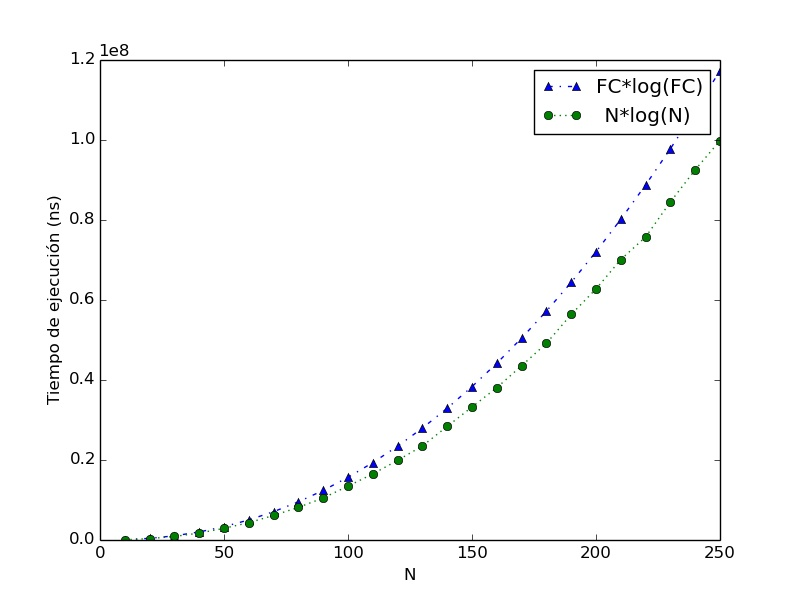
\includegraphics[width=0.6\textwidth]{sinParedes}
\caption{Aumento en la dimensión sel grafo}
\end{figure}

Podemos observar que el algoritmo tiene la misma tendencia logaritmica que nuestra cota teórica. También podemos ver que es mejor a media que aumenta la cantidad de nodos (o filas y columnas).


En este experimento mantuvimos o bien constante el número de filas para aumentar de 10 en 10 las columnas hasta 250, o bien el número de columnas para aumentar las filas.

\clearpage
\begin{figure}[!ht]
    \centering
    \begin{subfigure}{0.45\textwidth}
        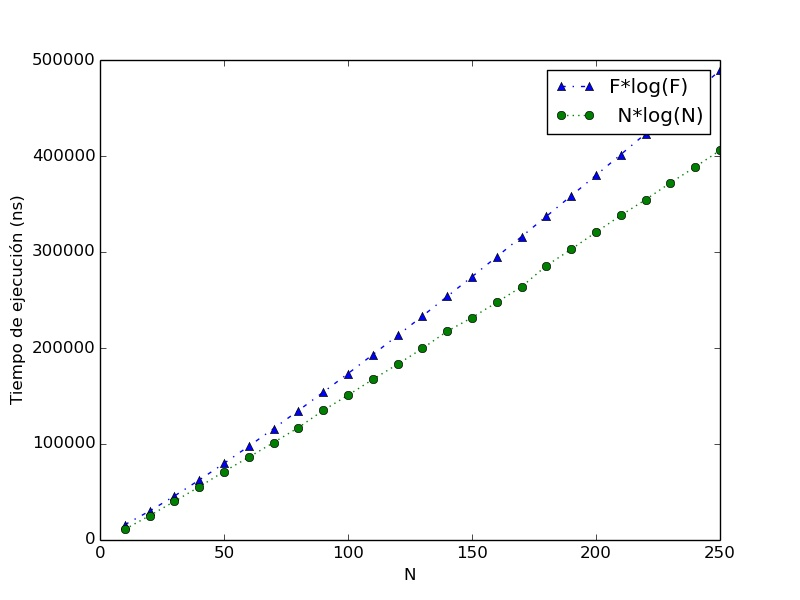
\includegraphics[width=\textwidth]{soloFilas}
        \caption{Aumento en filas del mapa.}
        \label{}
    \end{subfigure}
    \begin{subfigure}{0.45\textwidth}
        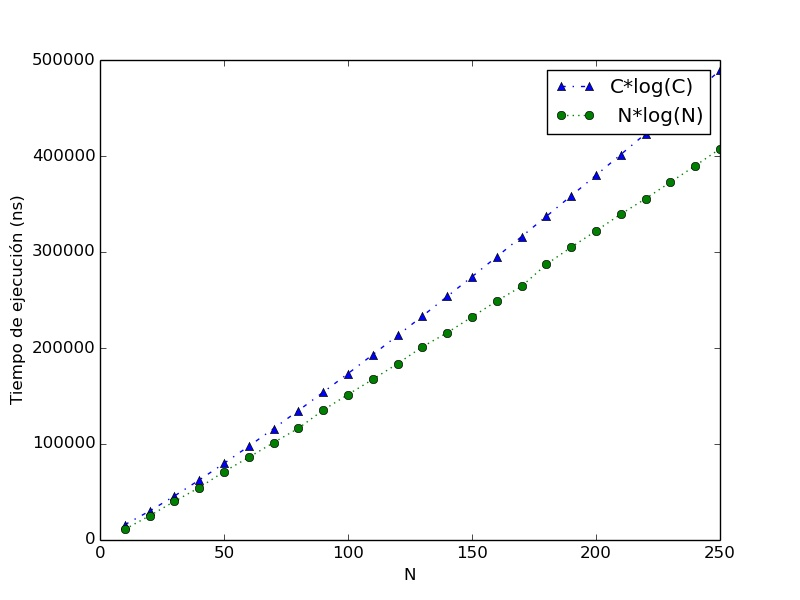
\includegraphics[width=\textwidth]{soloColumnas}
        \caption{Aumento en columnas del mapa.}
        \label{}
    \end{subfigure}
\end{figure}


Podemos ver que estos gráficos son practicamente iguales. con esto podemos mostrar que el algoritmo no depende en realidad de la cantidad de filas o columnas sino de los nodos. La razón por la cual nuestros gáficos son iguales es que mantienen la misma cantidad de nodos. la única diferencia en nustros mapas sería que uno es vertical y otro horizontal pero eso no afecta la cantidad de nodos.


Para este experimento creamos dos matrices manteniendo en una constante C=4 (habiendo entonces dos columnas de nodos) y en la otra C=6(habiendo 4 columnas de nodos). Fuimos aumentando las filas según como correspondiera en cada caso para mantener siempre la misma cantidad de nodos en ambos grafos.
\begin{figure}[H]
\centering
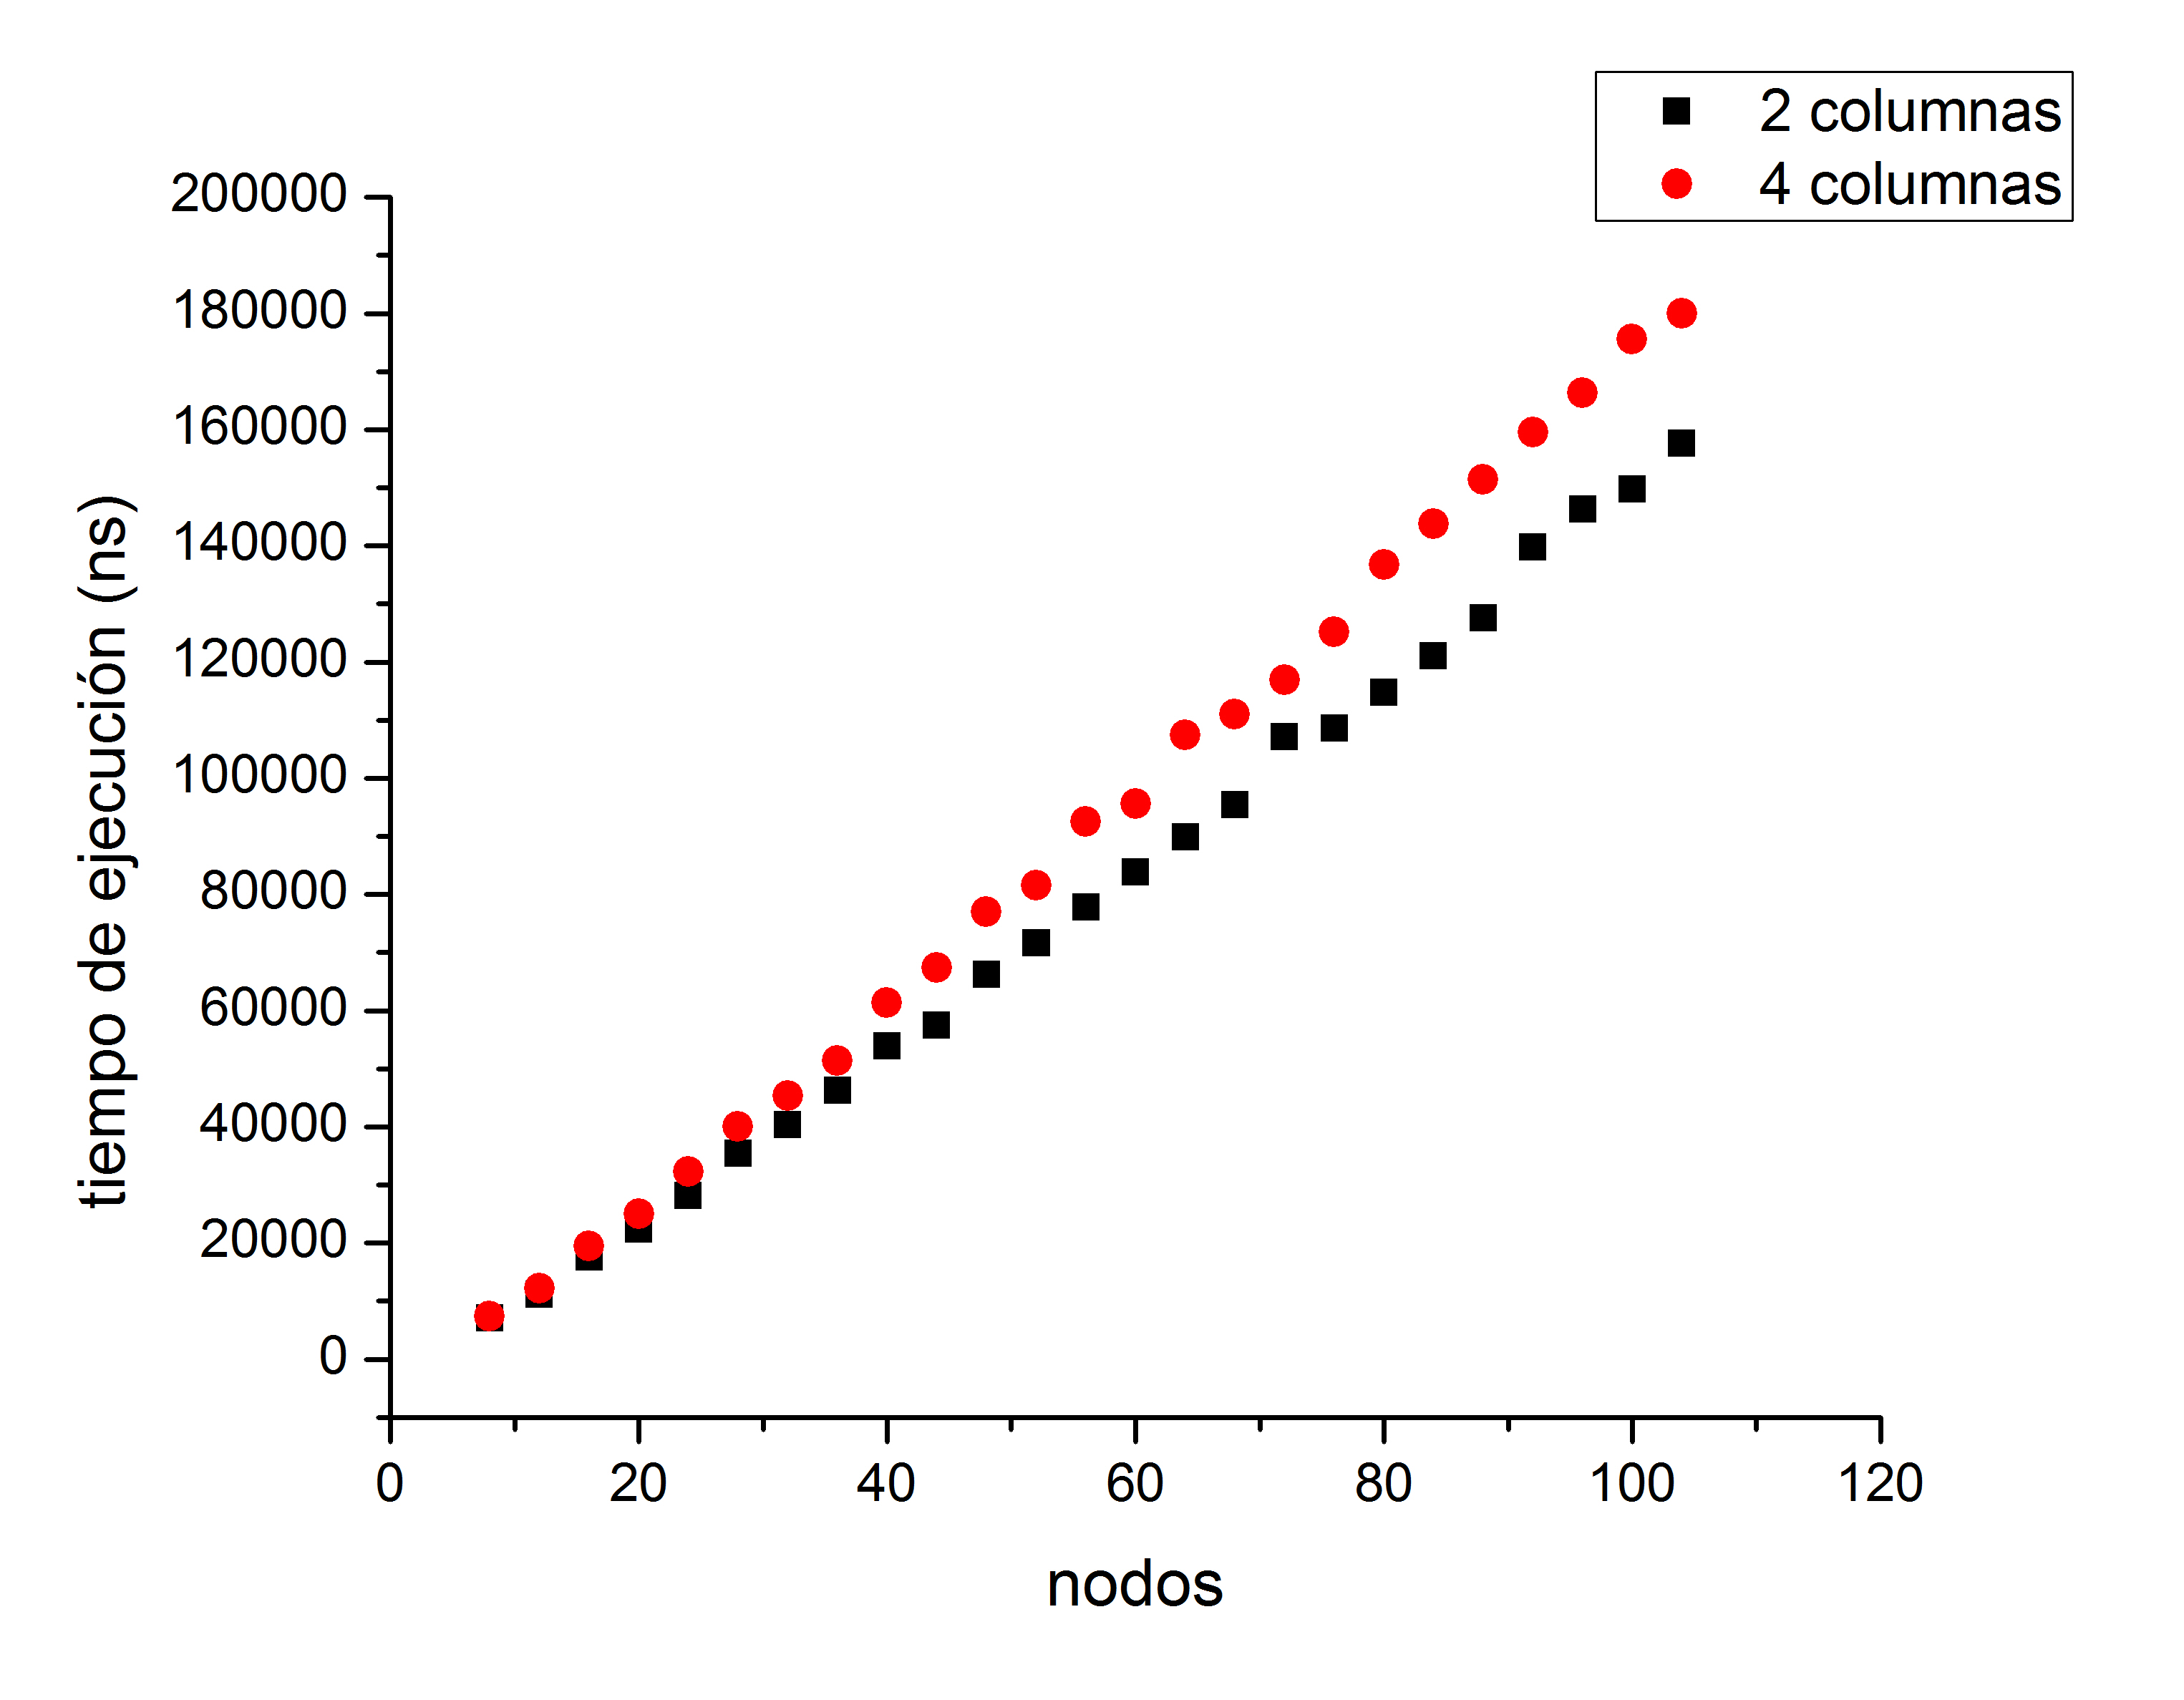
\includegraphics[width=0.6\textwidth]{2columvs4colum}
\caption{msima cantidad de nodos en mapas con distinta distribución}
\end{figure}

Podemos ver que el caso de 4 columnas tiene un tiempo de ejecución mayor. Esto se debe a que el algoritmo Kruskal tiene complejidad $\mathcal{O}(mxlog(n))$ y aunque en nuestro algoritmo podamos acotar la cantidad de ejes por la cantidad de nodos, esta diferencia sigue siendo perceptible como podemos observar en la figura. El grafo con 4 columnas tiene más ejes que el grafo con 2 pueso que los nodos del medio contienen cuatro ejes mientras que en el de 2 columnas la máxima cantidad de ejes que se puede aspirar a tener es 3 en los nodos que no son vértices.


En este experimentos tomamos un mapa con F=C=31 y fuimos aumentando las componentes  conexas, agregando alternadamente una columna de $"#"$ en el mapa.
\begin{figure}[H]
\centering
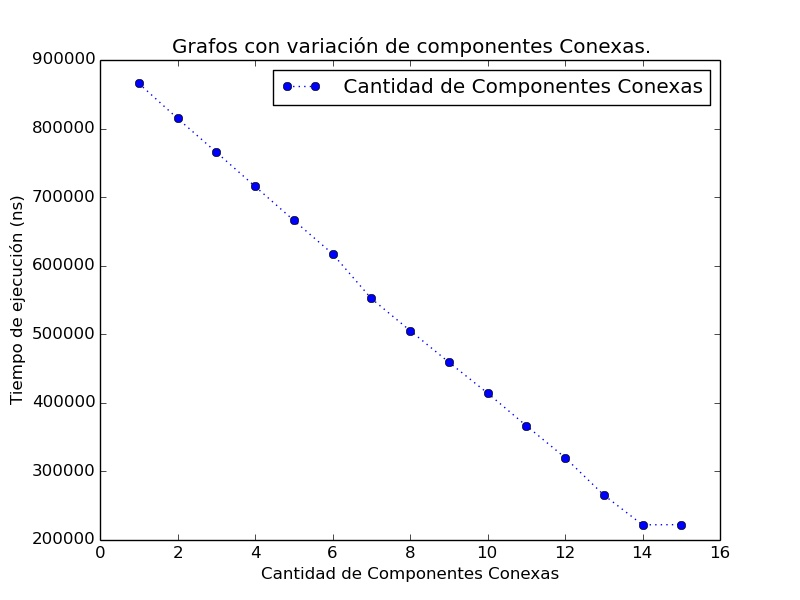
\includegraphics[width=0.6\textwidth]{CompConexas}
\caption{Aumento de las componentes conexas del grafo}
\end{figure}

Como podemos observar en esta figura el tiempo de ejecución disminuye a medida que aumentan las componentes conexas. Creemos que esto se debe a la disminusión de la cantidad de ejes por nodo, similar a como explicamos en la experimento anterior.






\section{Problema 3: Escapando}

\subsection{Introducción}

En este problema, los exploradores se encuentran en un dilema, luego de romper varias paredes la fortaleza se esta derrumbando. Por suerte ellos se encuentran en una habitación que tiene varios carritos y un mapa que les indica que estaciones estan conectadas y cuanto tardan en llegar de estación a estación. Lo que quieren es la forma más rápida de llegar desde el lugar en donde estan hasta la salida, que sería la última estación.

Formalmente, tenemos un digrafo rotulado, con peso en los ejes, y cada nodo esta identificado por un número desde el uno hasta la cantidad de nodos. Nuestro objetivo es encontrar el camino mínimo, dando el tiempo y su conjunto de nodos.


\subsection{Explicación de la solución}

   En esta sección explicaremos por que el problema dado se puede adapatar al algoritmo de camino mínimo de Dijkstra.
 La precondición que el algoritmo pide es que no tenga ejes negativos. Como el peso de los ejes esta definido como el tiempo que se tarda de llegar del nodo de origen al nodo de llegada podemos asegurarnos que nunca vamos a tener una entrada, que nos importe, que tenga un eje con peso negativo.

\subsubsection{Pseudocódigo}

\begin{algorithm}[H]{\textbf{CaminoMinimo}(MatrizAdy: Matriz(Nat, Nat) , estaciones: vector$<$Nat$>$)}
	\begin{algorithmic}[1]

		\State n $\gets$ tamaño(MatrizAdy)
		\State NodosSeguros $\gets$ 1
		\State nodosNoSeguros $\comment$ conjunto $\{$2, ..., n$\}$
		\State mientras NodosSeguros $\neq$ G
		\State \quad nodomin $\gets$ buscarMin(nodos, MatAdy[1])
		\State \quad nodosNoSeguros - $\{$nodomin$\}$
		\State \quad NodosSeguros $\cup$ $\{$nodomin$\}$
		\State \quad \forall \ e \ $\in$ nodos $\land$ [nodomin, e] $\in$ X
		\State \qquad longi $\gets$ $\pi_{1}$(matAdy[1][e])
		\State \qquad longmin $\gets$ $\pi_{1}$(matAdy[1][nodomin])
		\State \qquad longimin $\gets$ $\pi_{1}$(matAdy[nodomin][pos])
\\
		\qquad \textbf{if} longi $\geq$ longmin +longimin
			\State \qquad \quad matAdy[1][e] $\gets$ (longpmin + longimin, nodomin)
\\
 \qquad \textbf{endif}

		\State tiempo $\gets$ $\pi_{1}$(MatAdy[1][n])
		\State pred $\gets$ n
		\State mientras pred $\neq$ 1 \ $\land$ \ pred $\neq$ 0 (cuando no existe camino)
		\State \quad estaciones $\cup$ $\{$pred$\}$
		\State \quad pred $\gets$ $\pi_{2}$(matAdy[1][pred])

		\State res $\gets$ tiempo
 	\end{algorithmic}
\end{algorithm}

\begin{algorithm}[H]{\textbf{CaminoMinimo}(mochilas: vector$<$mochila$>$, cofre: vector$<$tesoro$>$)}
	\begin{algorithmic}[1]

		\State sol$\gets$ ValorOptim
	\end{algorithmic}
\end{algorithm}

\newpage

\subsubsection{Demostración de Correctitud}
Como podemos apreciar el pseudocódigo es el algoritmo Dijsktra, entonces su correctitud se desprende de la demostración de correctitud de dijkstra que se puede encontrar en varios libros de algoritmos, en nuestro caso vamos a referenciar al libro titulado ``Introduction to Algorithms, Second Edition"  de Thomas H Cormen, Charles E. Leiserson, entre otros. La demostracion se encuentra en el capítulo 24, subsección 3 bajo el título ``Theorem 24.6: (Correctness of Dijkstra's algorithm)".

\subsubsection{Demostración de Complejidad}

%No pude tabular, ni con \quad ni con \tab ni con $\>$ ni con $\-$ pero parece ser un problema de el salto de linea.
Si analizamos con atención el pseudocódigo, Tenemos tres secciones que se pueden analizar por separado y despues sumar sus complejidades nos dara la complejidad total del algoritmo. La primer parte y la segunda parte combinadas son Dijkstra, la primera es la creación de la matriz y la segunda son los cálculos, La tercer parte es poner la información del camino mínimo. En los próximos párrafos nos vamos a referir a la cantidad de nodos en el gráfico como N.
\\
	 La primer parte a analizar es la creación de la matriz, al ser una matriz de adyacencia, la cantidad de filas es N y la cantidad de columnas es N, actualizar todos los valores es recorrer toda la matriz haciendo que la complejidad sea $\Theta$(N²)
\\
	La segunda parte son dos ciclos anidados, podemos observar que el ciclo exterior hace N iteraciones ya que termina cuando el conjunto de nodos del grafo tiene el mismo cardinal que el conjunto de ``nodosSeguros'' y este último aumenta en uno por cada iteración. Dentro del ciclo principal tenemos dos operaciones que debemos tener en cuenta, sacar el nodo de la lista de ``nodosNoSeguros'' y el ciclo interno. Sacar un nodo de la lista, nos va a costar encontrar el nodo y luego eliminarlo. Por la estructura que utlizamos eliminarlo no nos aporta complejidad, pero encontrar el nodo es una busqueda lineal, es decir $\mathcal{O}$(N). La última parte que nos falta analizar para poder determinar la complejidad de los ciclos anidados es el ciclo interno. Cada iteración recorre N posiciones de la matriz, aquellas que podrían ser un eje válido, aunque hace cosas dependiendo de si es un eje válido o no, el interior del ciclo aporta una complejidad constante. Reuniendo toda la información, el interior del ciclo externo nos aporta una complejidad $\mathcal{O}$(N) y itera N veces, es decir que la complejidad de la segunda parte es $\mathcal{O}$(N²).
\\
	 La tercer parte es un ciclo que lee los datos de la matriz y guarda en un conjunto los nodos que tenemos que atravezar para tener el camino mínimo. La cantidad máxima de iteraciones que hace este ciclo es N, el razonamiento atras de esta afirmación es que los ejes no tienen pesos negativos, si existe un camino mínimo, este no va a tener ciclos ya que pasar por un ciclo solo aumentaría el peso total del camino, y un camino sin ciclos en un grafo con n nodos tiene como mucho n-1 ejes, ya que el camino puede llegar a pasar por todos los nodos. Podemos concluir que el ciclo hace n iteraciones en el peor caso, es decir que la tercer parte es $\mathcal{O}$(N)
\\
\tab Ahora que analizamos las tres partes que podían llegar a dar complejidad al algoritmo sabemos que la complejidad algoritmica de la primer parte, la segunda parte y la tercera respectivamente son $\Theta$(N²), $\mathcal{O}$(N²), $\mathcal{O}$(N). Entonces la complejidad total es la suma de las complejidades dandonos $\mathcal{O}$(N²).

\subsection{Experimentación}

La cota de complejidad de nuestro algoritmo es $\mathcal{O}$(N²). Es decir que depende de la cantidad de nodos en un grafo.
En esta sección trataremos de respaldar esta cota mediante el análisis de los datos empíricos que obtuvimos a traves del testeo de nuestros algoritmos.
\\
Tenemos dos algoritmos, los dos una variación del mismo pseudocódigo, el algoritmo sin modificaciones, A1, este busca el camino mínimo con todos los nodos y el algoritmo, A2, este se interrumpe cuando encuentra el camino mínimo que estamos buscando.
\\
 Decidimos testear sobre los dos algoritmos ya que al asignar peso aleatorio a los ejes en la mayoría de los casos teníamos la intuición de que los gráficos podrían quedar bastante mal. Pensamos en hacer test donde nos asegurabamos que se recorrían todos los nodos, pero al final decidimos usar dos variaciones del mismo algoritmo. Esto nos va a ayudar a demostrar que el algoritmo que nosotros elejimos en el peor caso tiene una complejidad igual al que realmente nos va a probar la cota N² y en el mejor caso tiene una complejidad lineal.
\\
Con este objetivo a lo largo de los tests modificamos los grafos para observar su comportamiento y poder sacar conclusiones sobre las elecciones algoritmicas que tomamos. En cada test los valores se logran al promediar un tres mil iteraciones sobre el mismo input, sobre que forma tiene el input se va a hablar más adelante.

\subsubsection{Resultados y análisis}

En nuestro primer experimento corrimos el algoritmo con diferentes grafos Kn, donde el n empieza en diez, se incrementa por diez y termina en 250 y los pesos de los ejes se generan de forma aleatoria. Creamos estos parametros para tener una primera impresión de como variaba dependiendo solamente de los nodos, ya que los ejes depende de la cantidad de nodos. Nuestra expectativa era que A1 tenga un comportamiento cuadrático y que A2 tenga un comportamiento errático pero parecido a una función cuadrática, ya que no sabíamos como iban a afectar la interrupciones que metimos en el algoritmo, esperabamos mejoras en algunas iteraciones.

\begin{figure}[H]
\centering
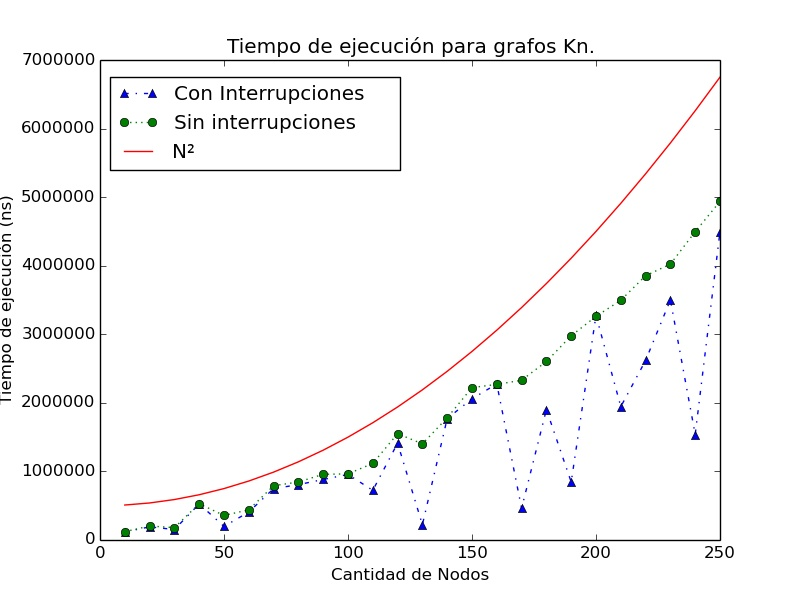
\includegraphics[width=0.6\textwidth]{KnC100r3000}
\caption{}
\end{figure}

Como se puede ver en el gráfico, nuestras expectativas fueron cumplidas, A1 tiene un tendencia cuadrática y A2 aunque no muestra una tendencia clara esta por debajo de A1. Como explicamos anteriormente este comportamiento errático responde a que A2 frena cuando encuentra el camino mínimo para n y no sigue ejecutando para otros nodos, esto quiere decir que cuanto más cerca esta A1 de A2 es que el camino mínimo de n es uno de los últimos en computarse y analogamente si estan lejos es que n es uno de los primeros en computarse.
\\
Al encontar respaldo empírico sobre como nuestro algoritmo cumple con las complejidades teóricas, decidimos evaluar como respondia A1 y A2 sobre el mejor caso, este seria que el camino mínimo sea el eje que va desde 1 hasta n, ya que A2 corta en cuanto encuentra la solución para n. Nuestra complejidad, despues de leer el input es lineal. Lo que creamos es un test que nos crea grafos Kn y que tienen la particularidad de que el eje (1,n) pesa cero, haciendolo el camino mínimo. Debajo se encuentran dos gráficos que modelan este test.

\begin{figure}[H]
\centering
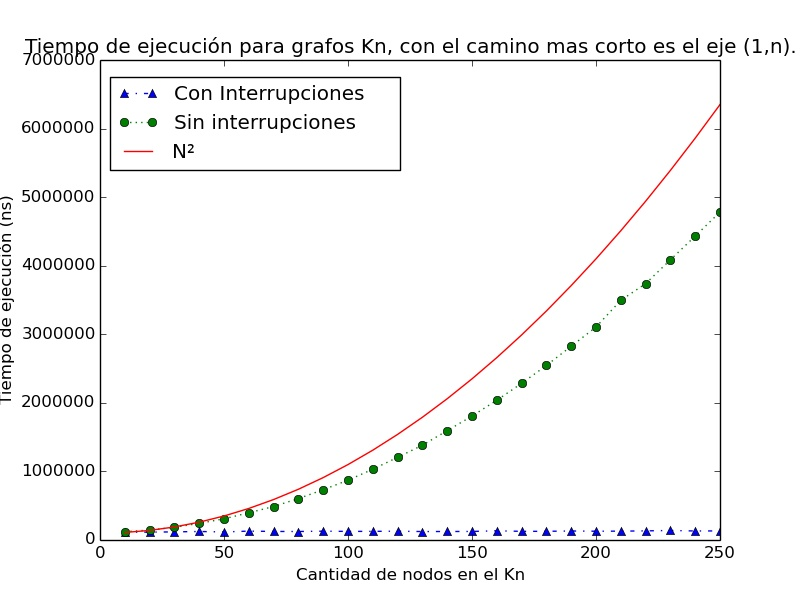
\includegraphics[width=0.6\textwidth]{KnOptC150r3000}
\caption{}
\end{figure}
\\
En este gráfico podemos ver como A1 mantiene su apariencia cuadratica, pero nos hace pensar que A2 tiene una forma constante, lo cual no nos resulto coherente  por lo que nosotros sabemos de la implementación, la busqueda lineal del mínimo tiene que seguir ocurriendo. Por eso decidimos mirar solo la línea de A2 para ver que a que función se asemejaba.


\begin{figure}[H]
\centering
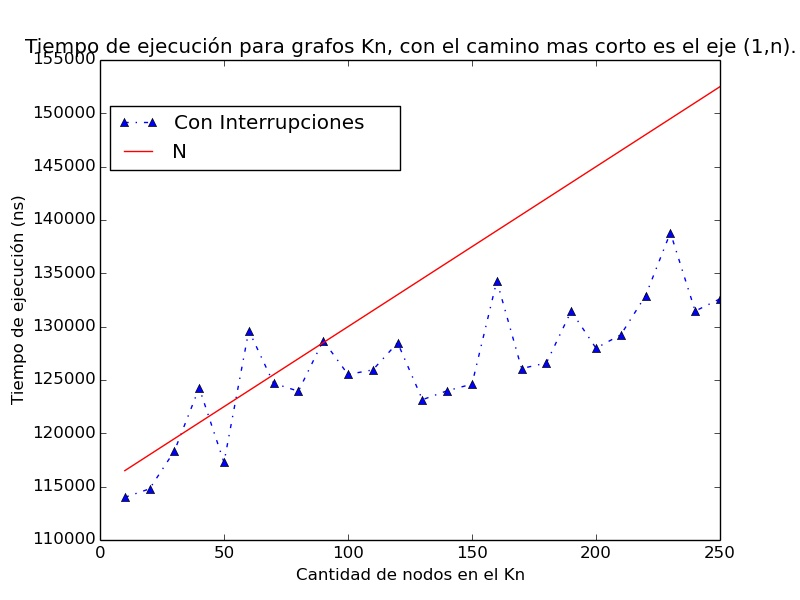
\includegraphics[width=0.6\textwidth]{KnsoloOptC100r3000}
\caption{}
\end{figure}
\\
Como Podemos observar la apariencia constante de A2 era meramente una apariencia por las escalas que tenía la figura 2. Ahora se nota claramente que A2 en el mejor caso es lineal.
\\
Al finalizar estos experimentos, nos dimos cuenta que modificar la cantidad de nodos y que la cantidad de ejes este en función a la cantidad de nodos nos reducía el univierso de posibles grafos y en ese sentido por ahí habían dependencias en terminos de complejidad que nosotros no cubríamos.
\\
 Entonces creamos este experimento, que crea grafos conexos con 200 ejes y varía los nodos desde 20 hasta 199 y los pesos estan asignados aleatoriamente. Esperabamos un gráfico muy parecido a la figura 1.

\begin{figure}[H]
\centering
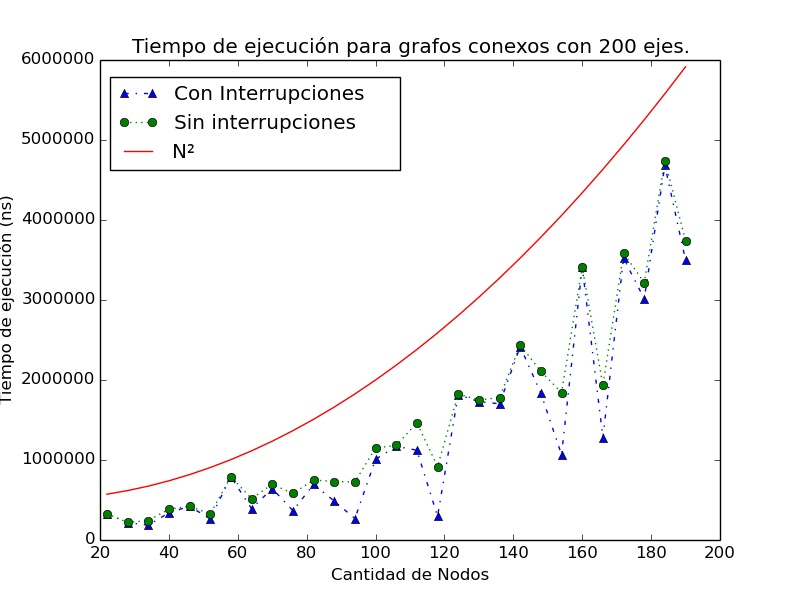
\includegraphics[width=0.6\textwidth]{Conexo200ejesC150r3000}
\caption{}
\end{figure}

Aunque se pueden ver unas tendencias cuadráticas en el gráfico y que esta por debajo de la cota dada, tambien podemos ver que la figura 1 tiene los datos de A1 más regulares que en la figura 2. Nuestras hipótesis es que cuanto más denso es el grafo, más regular quedan las mediciones y cuanto menos denso las mediciones tienden a ser irregulares. Entonces decidimos experimentar sobre grafos menos densos y ver como quedaban las mediciones.
\\
A fin de lo antes mencionado creamos una prueba, que dada una cierta cantidad de nodos, nos generaba cuatro grafos. Definimos el concepto D, como una simil densidad, donde la densidad esta definida como la cantidad de ejes en un grafo dado, cuanto más denso el grafo más ejes tiene. D funciona solo para grafos conexos, 0 es un árbol y 100 es el Kn.

\begin{figure}[H]
\centering
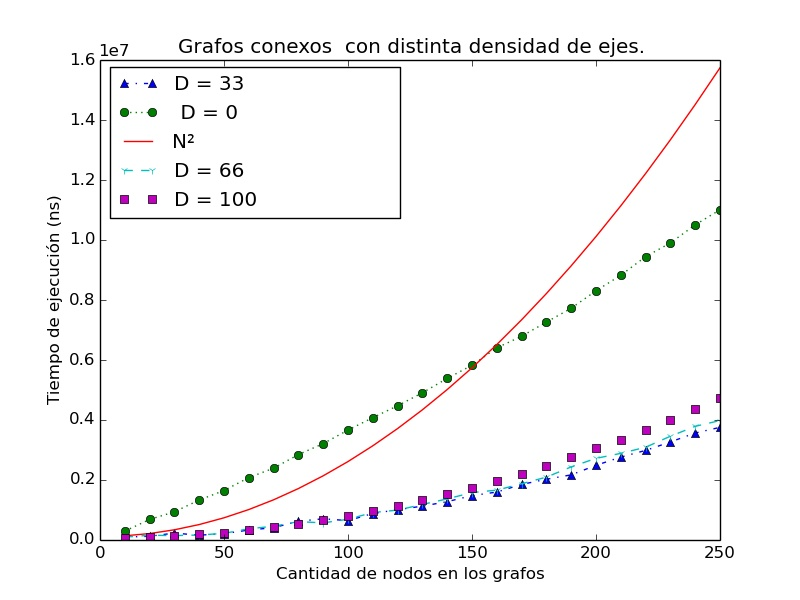
\includegraphics[width=0.6\textwidth]{VariasDensidades}
\caption{}
\end{figure}

Como se puede observar en el gráfico no respalda nuestra hipótesis, y nos genera una incertidumbre aún mayor, al encontrar la línea de Arboles muy por encima de las otras tres, que no era la idea intuitiva que nosotros teníamos donde los grafos menos densos iban a estar acotados por grafos más densos. Aun así el próximo el gráfico sin los arboles avala esta idea y podríamos pensar que el caso de los arboles es una excepción a la regla.

\begin{figure}[H]
\centering
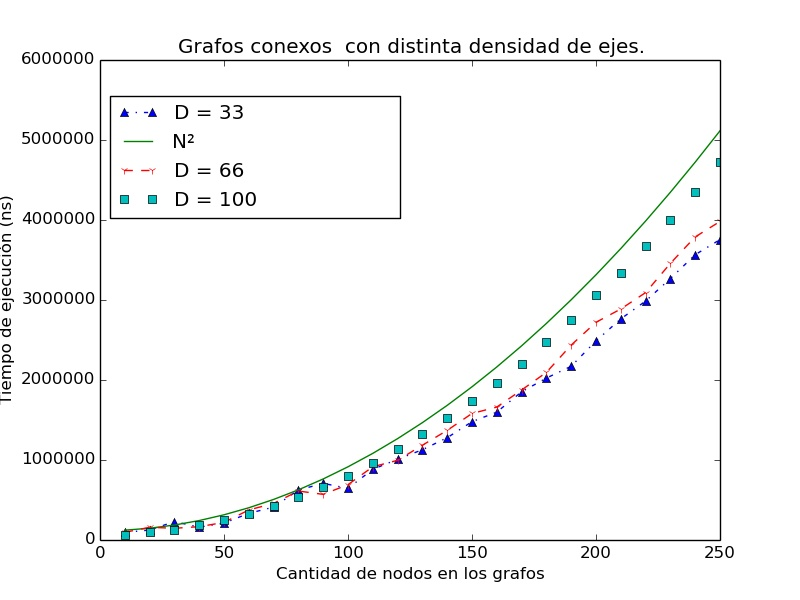
\includegraphics[width=0.6\textwidth]{VariasDensidadesSinArbol}
\caption{}
\end{figure}

\\
Luego de demostrar que la complejidad Teórica es respaldada por la experimentación, entramos en una series de pruebas que se generaron más por la falta de entendimiento de nuestros gráficos y la busqueda de una hipótesis que satisfaga al lector. Lamentablemente no encontramos una, solo encontramos más preguntas sin resolver, que para no agobiar al lector dejamos como meras incognitas para encarar en un futuro.¿Por qué los árboles tardan una cantidad significante más de tiempo que un grafo fuertemente conexo?¿Como se explica la variación de tiempos cuando la cantidad de ejes es lo mismo pero los nodos aumentan? Acaso fue que las 3000 iteraciones dieron unas mediciones poco estandares o hay una razon por la cual un grafo con 124 nodos tenga el mismo tiempo de ejecucion que un de 170, cuando estos tendrian que ser muy diferentes.


\end{document}
